\let\lesson\undefined
\newcommand{\lesson}{\phantomlesson{Bài 10.}}
\setcounter{section}{2}
\section{Bài tập trắc nghiệm}
\begin{enumerate}[label=\bfseries Câu \arabic*:,leftmargin=1.5cm]
	\item \mkstar{1}\\
	{Trong chuyển động thẳng biến đổi đều, gia tốc
		\begin{mcq}(2)
			\item có giá trị bằng 0.
			\item là một hằng số khác 0.
			\item có giá trị biến đổi theo thời gian.
			\item chỉ thay đổi hướng chứ không thay đổi về độ lớn.
		\end{mcq}
	
}
\hideall{
\textbf{Đáp án: B.}
}

\item \mkstar{1}\\
{Một xe máy đang đứng yên, sau đó khởi động và bắt đầu tăng tốc. Nếu chọn chiều dương là chiều chuyển động của xe thì nhận xét nào sau đây là đúng?
	\begin{mcq}(4)
		\item $a>0$, $v>0$.
		\item $a>0$, $v<0$.
		\item $a<0$, $v>0$.
		\item $a<0$, $v<0$.
	\end{mcq}

}
\hideall{
\textbf{Đáp án: A.}
}

\item \mkstar{1}\\
{Trong các đồ thị vận tốc - thời gian dưới đây, đồ thị nào mô tả chuyển động thẳng biến đổi đều?
	\begin{center}
		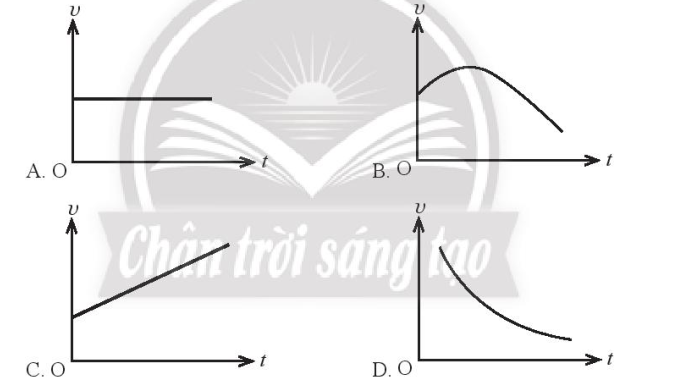
\includegraphics[width=0.7\linewidth]{../figs/VN10-2023-PH-TP0003-1}
	\end{center}

}
\hideall{
\textbf{Đáp án: C.}
}

\item \mkstar{1}\\
{Trong các phương trình mô tả vận tốc $v \left(\si{\meter/\second}\right)$ của vật theo thời gian $t \left(\si{\second}\right)$ dưới đây, phương trình nào mô tả chuyển động thẳng biến đổi đều?
	\begin{mcq}(4)
		\item $v=7$.
		\item $v=6t^2+2t-2$.
		\item $v=5t-4$.
		\item $v=6t^2-2$.
	\end{mcq}

}
\hideall{
\textbf{Đáp án: C.}
}

\item \mkstar{1}\\
{Vật A có khối lượng gấp hai lần vật B. Ném hai vật theo phương ngang với cùng tốc độ đầu ở cùng một vị trí. Nếu bỏ qua mọi lực cản thì
	\begin{mcq}
		\item vị trí chạm đất của vật A xa hơn vị trí chạm đất của vật B.
		\item vị trí chạm đất của vật B xa hơn vị trí chạm đất của vật A.
		\item vật A và B rơi cùng vị trí.
		\item chưa đủ dữ kiện để đưa ra kết luận về vị trí của hai vật.
	\end{mcq}

}
\hideall{
\textbf{Đáp án: C.}\\
Nếu bỏ qua mọi lực cản thì tầm ném xa của vật:
$$L=v_0\cdot\sqrt{\dfrac{2H}{g}}$$
Nếu hai vật được ném từ cùng độ cao với cùng tốc độ đầu thì hai vật chạm đất ở cùng vị trí.
}

\item \mkstar{1}\\
{Đồ thị nào sau đây là của chuyển động biến đổi?
\begin{center}
	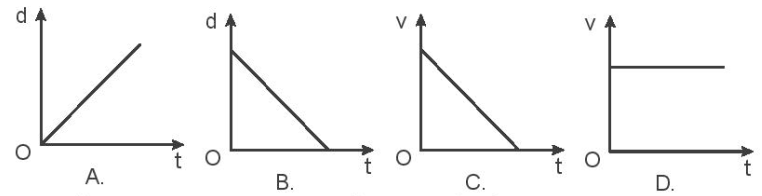
\includegraphics[width=0.7\linewidth]{../figs/VN10-2023-PH-TP0003-5}
\end{center}

}
\hideall{
\textbf{Đáp án: C.}
}

\item \mkstar{1}\\
{Đồ thị vận tốc - thời gian nào sau đây mô tả chuyển động có độ lớn gia tốc là lớn nhất?
	\begin{center}
		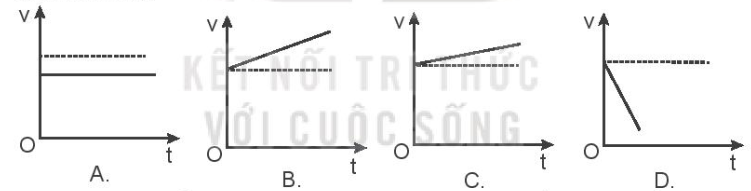
\includegraphics[width=0.7\linewidth]{../figs/VN10-2023-PH-TP0003-6}
	\end{center}

}
\hideall{
\textbf{Đáp án: D.}
}

\item \mkstar{1}\\
{Chuyển động nào sau đây không phải là chuyển động thẳng biến đổi đều?
	\begin{mcq}(2)
		\item Viên bi lăn xuống máng nghiêng.
		\item Vật rơi từ trên cao xuống đất.
		\item Hòn bi bị ném theo phương nằm ngang.
		\item Quả bóng được ném lên theo phương thẳng đứng.
	\end{mcq}

}
\hideall{
\textbf{Đáp án: C.}\\
Vật bị ném ngang chuyển động theo quỹ đạo cong.
}

\item \mkstar{1}\\
{Công thức liên hệ giữa độ dịch chuyển, vận tốc và gia tốc của chuyển động nhanh dần đều là
	\begin{mcq}(4)
		\item $v^2-v^2_0=ad$.
		\item $v^2-v^2_0=2ad$.
		\item $v-v_0=ad$.
		\item $v^2_0-v^2=2ad$.
	\end{mcq}

}
\hideall{
\textbf{Đáp án: B.}
}

\item \mkstar{1}\\
{Đồ thị nào sau đây mô tả chuyển động thẳng chậm dần đều?
	\begin{center}
		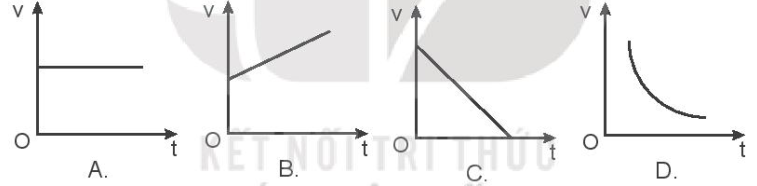
\includegraphics[width=0.7\linewidth]{../figs/VN10-2023-PH-TP0003-7}
	\end{center}

}
\hideall{
\textbf{Đáp án: C.}
}

\item \mkstar{2}\\
{Chuyển động của vật nào dưới đây sẽ được coi là rơi tự do nếu được thả rơi?
	\begin{mcq}(4)
		\item Một khăn voan nhẹ.
		\item Một sợi chỉ.
		\item Một chiếc lá.
		\item Một viên sỏi.
	\end{mcq}

}
\hideall{
\textbf{Đáp án: D.}
}


\item \mkstar{2}\\
{	Quan sát đồ thị vận tốc - thời gian (hình bên) của một vật đang chuyển động thẳng và cho biết quãng đường vật đi được trong khoảng thời gian nào là lớn nhất?\\
	\begin{minipage}[l]{0.6\textwidth}
	\begin{mcq}
		\item Trong khoảng thời gian từ 0 đến $\SI{1}{\second}$.
		\item Trong khoảng thời gian từ $\SI{1}{\second}$ đến $\SI{2}{\second}$.
		\item Trong khoảng thời gian từ $\SI{2}{\second}$ đến $\SI{3}{\second}$.
		\item Trong khoảng thời gian từ $\SI{3}{\second}$ đến $\SI{4}{\second}$.
	\end{mcq}
	\end{minipage}
	\begin{minipage}{0.4\textwidth}
		\begin{center}
			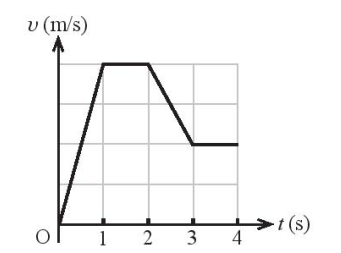
\includegraphics[width=0.6\linewidth]{../figs/VN10-2023-PH-TP0003-2}
		\end{center}
	\end{minipage}

}
\hideall{
\textbf{Đáp án: B.}
}

\item \mkstar{2}\\
{	Hình bên mô tả đồ thị $\left(v-t\right)$ của bốn xe ô tô A, B, C, D. Nhận định nào sau đây là đúng?
	\begin{center}
		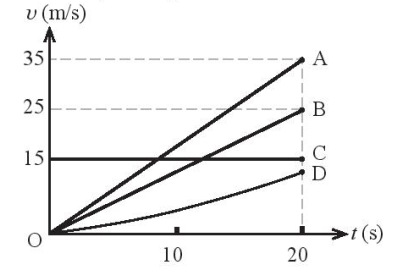
\includegraphics[width=0.4\linewidth]{../figs/VN10-2023-PH-TP0003-3}
	\end{center}
	\begin{mcq}
		\item Xe C chuyển động đều, còn các xe còn lại là chuyển động biến đổi đều.
		\item Xe C chuyển động đều và chỉ có chuyển động của xe A là biến đổi đều.
		\item Chỉ có xe A và B chuyển động biến đổi đều, xe C chuyển động đều.
		\item Chỉ có xe D chuyển động biến đổi đều, xe C chuyển động đều.
	\end{mcq}

}
\hideall{
\textbf{Đáp án: A.}
}

\item \mkstar{2}\\
{Trong tiết học Vật lí, ba bạn Mi, Hiếu và Đức tranh luận về thời gian rơi của vật chuyển động ném ngang so với vật thả rơi tự do khi ở cùng một độ cao và bỏ qua mọi lực cản. Bạn Mi cho rằng: "Khi ném một vật theo phương ngang thì vật sẽ chuyển động lâu hơn so với việc thả rơi tự do vì khi ném ngang, vật sẽ đi quãng đường dài hơn". Bạn Hiếu lại có ý kiến khác: "Thời gian rơi của hai vật là bằng nhau vì trong cả hai trường hợp, tính chất chuyển động của vật theo phương thẳng đứng là như nhau". Còn bạn Đức thì cho rằng: "Thời gian rơi khi vật chuyển động ném ngang còn phụ thuộc vào vận tốc ban đầu nên không thể kết luận về thời gian rơi trong hai trường hợp này". Theo em, bạn nào đưa ra ý kiến đúng?
	\begin{mcq}(2)
		\item Bạn Mi.
		\item Bạn Hiếu.
		\item Bạn Đức.
		\item Cả ba bạn đều không chính xác.
	\end{mcq}

}
\hideall{
\textbf{Đáp án: B.}
}

\item \mkstar{3}\\
{Xét hai xe A và B chuyển động cùng nhau vào hầm Thủ Thiêm dài $\SI{1490}{\meter}$. Xe A chuyển động với tốc độ ban đầu trước khi vào hầm là $\SI{60}{\kilo\meter/\hour}$ và chuyển động chậm dần đều với gia tốc $\SI{144}{\kilo\meter/\hour^2}$, xe B chuyển động chậm dần đều với gia tốc $\SI{120}{\kilo\meter/\hour^2}$ từ lúc bắt đầu chạy vào hầm với tốc độ $\SI{55}{\kilo\meter/\hour}$. Nhận định nào sau đây là đúng về thời gian chuyển động của hai xe trong hầm?
	\begin{mcq}
		\item Hai xe đi hết hầm Thủ Thiêm cùng một khoảng thời gian.
		\item Xe B ra khỏi hầm trước xe A.
		\item Xe A ra khỏi hầm trước xe B.
		\item Dữ liệu bài toán không đủ kết luận.
	\end{mcq}

}
\hideall{
\textbf{Đáp án: C.}\\
Thời gian chuyển động của xe A:
$$s=v_{0A}t-\dfrac{1}{2}a_At^2\Rightarrow t=\SI{0.8}{\hour}$$
Thời gian chuyển động của xe B:
$$s=v_{0B}t-\dfrac{1}{2}a_Bt^2\Rightarrow t=\SI{0.89}{\hour}$$
Như vậy, xe A ra khỏi hầm trước xe B.
}

\item\mkstar{3}\\
{Một vật được ném từ độ cao $H$ với vận tốc ban đầu $v_0$ theo phương nằm ngang. Nếu bỏ qua sức cản của không khi thì tầm xa $L$
	\begin{mcq}(2)
		\item tăng 4 lần khi $v_0$ tăng 2 lần.
		\item tăng 2 lần khi $H$ tăng 2 lần.
		\item giảm 2 lần khi $H$ giảm 4 lần.
		\item giảm 2 lần khi $v_0$ giảm 4 lần.
	\end{mcq}

}
\hideall{
\textbf{Đáp án: C.}\\
Tầm xa:
$$L=v_0\cdot\sqrt{\dfrac{2H}{g}}$$
Khi $H$ giảm 4 lần thì tầm xa giảm 2 lần.
}
\item\mkstar{3}\\
{Thả một hòn sỏi từ độ cao $h$ xuống đất. Hòn sỏi rơi trong $\SI{2}{\second}$. Nếu thả hòn sỏi từ độ cao $2h$ xuống đất thì hòn sỏi rơi trong bao lâu?
	\begin{mcq}(4)
		\item $\SI{2}{\second}$.
		\item $\xsi{2\sqrt{2}}{\second}$.
		\item $\SI{4}{\second}$.
		\item $\xsi{4\sqrt{2}}{\second}$.
	\end{mcq}

}
\hideall{
\textbf{Đáp án: B.}\\
Thời gian rơi của vật rơi tự do:
$$t=\sqrt{\dfrac{2h}{g}}$$
Vì $h'=2h\Rightarrow t'=t\sqrt{2}=\xsi{2\sqrt{2}}{\second}$.
}

\item \mkstar{3}\\
{Một vật được thả rơi từ độ cao $\SI{9.8}{\meter}$ xuống đất. Bỏ qua lực cản của không khí. Lấy gia tốc rơi tự do $g=\SI{9.8}{\meter/\second^2}$. Tốc độ của vật trước khi chạm đất là
	\begin{mcq}(4)
		\item $\xsi{9,8\sqrt{2}}{\meter/\second}$.
		\item $\SI{9.8}{\meter/\second}$.
		\item $\SI{98}{\meter/\second}$.
		\item $\SI{6.9}{\meter/\second}$.
	\end{mcq}

}
\hideall{
\textbf{Đáp án: A.}\\
Tốc độ của vật trước khi chạm đất:
$$v=\sqrt{2gh}=\xsi{9,8\sqrt{2}}{\meter}.$$
}

\item \mkstar{3}\\
{Hai vật được ném đồng thời từ mặt đất lên với vận tốc ban đầu như hình vẽ. Nếu bỏ qua sức cản của không khí thì câu nào sau đây không đúng?\\
	\begin{minipage}[l]{0.6\textwidth}
		\begin{mcq}
			\item Hai vật chạm đất cùng lúc.
			\item Hai vật cùng có tầm bay xa.
			\item Vật 2 có tầm bay xa lớn hơn.
			\item Hai vật có cùng tầm bay cao.
		\end{mcq}
	\end{minipage}
\begin{minipage}{0.4\textwidth}
	\begin{center}
		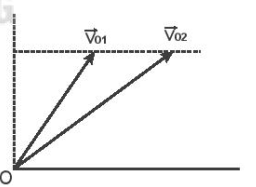
\includegraphics[width=0.6\linewidth]{../figs/VN10-2023-PH-TP0003-8}
	\end{center}
\end{minipage}
}
\hideall{
\textbf{Đáp án: B.}\\
Vì tốc độ ban đầu trên phương thẳng đứng của hai vật như nhau nên hai vật chạm đất cùng lúc (cùng thời gian chuyển động) $\Rightarrow$ A đúng.

Vì tốc độ ban đầu trên phương ngang của vật 2 lớn hơn tốc độ ban đầu trên phương ngang của vật 1 nên vật 2 có tầm xa lớn hơn $\Rightarrow$ B sai, C đúng.

Độ cao cực đại trong chuyển động ném xiên $H=\dfrac{v^2_{0y}}{2g}$. Vì tốc độ ban đầu của hai vật trên phương thẳng đứng bằng nhau nên hai vật có cùng tầm bay cao.
}

\item \mkstar{4}\\
{Một vận động viên sút một quả bóng bầu dục ba lần theo các quỹ đạo a, b, c như hình bên. Quỹ đạo nào tương ứng với thời gian chuyển động trong không khí của quả bóng là lâu nhất nếu bỏ qua mọi lực cản?
	\begin{center}
		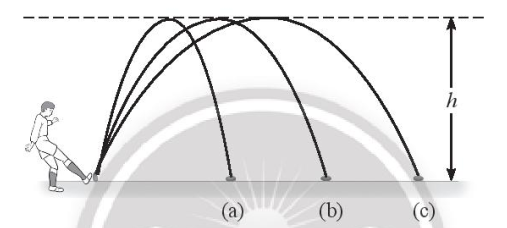
\includegraphics[width=0.4\linewidth]{../figs/VN10-2023-PH-TP0003-4}
	\end{center}
	\begin{mcq}(2)
		\item (a).
		\item (b).
		\item (c).
		\item Cả ba trường hợp có thời gian chuyển động như nhau.
	\end{mcq}

}
\hideall{
\textbf{Đáp án: D.}\\
Thời gian chuyển động của vật ném xiên từ mặt đất:
$$t=2\cdot \dfrac{v_{0y}}{g}$$
Ba lần sút quả bóng có cùng độ cao cực đại nên $v_{0y}$ trong 3 trường hợp là như nhau $\left(H=\dfrac{v^2_{0y}}{2g}\right)$. Từ đó suy ra thời gian chuyển động của quả bóng trong 3 trường hợp là như nhau.
}
\end{enumerate}
\section{Bài tập tự luận}
\begin{enumerate}[label=\bfseries Bài \arabic*:,leftmargin=1.5cm]
	\item \mkstar{2}\\
	{Khi dùng vòi nước tưới cây, để các tia nước phun ra xa, người ta thường điều chỉnh sao cho hướng của vòi xiên một góc nào đó với phương ngang. Trong trường hợp lý tưởng (bỏ qua mọi lực cản), góc hợp giữa vòi và phương ngang phải bằng bao nhiêu để các tia nước phun ra xa nhất?
		\begin{center}
			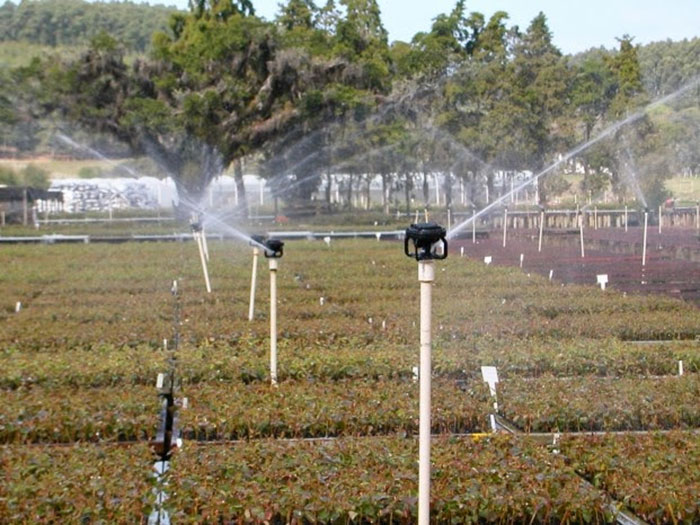
\includegraphics[width=0.3\linewidth]{../figs/VN10-2023-PH-TP0003-11}
		\end{center}
	
}
\hideall{
	Tầm xa của giọt nước:
	$$L=\dfrac{v^2_0\sin2\theta}{g}$$
	Giọt nước đạt tầm xa cực đại khi $\sin2\theta=1\Rightarrow \theta =\SI{45}{\degree}$.
}
	
	\item \mkstar{2}\\
	{Quan sát đồ thị vận tốc - thời gian mô tả chuyển động của một tàu hoả và trả lời các câu hỏi sau:
		\begin{center}
			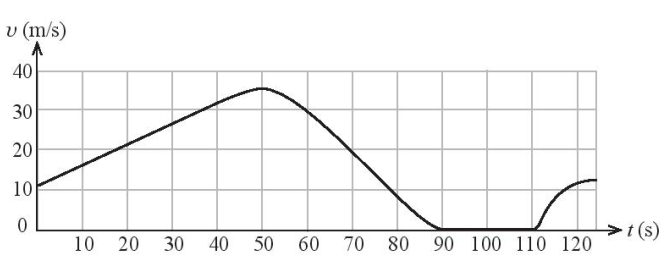
\includegraphics[width=0.6\linewidth]{../figs/VN10-2023-PH-TP0003-9}
		\end{center}
	\begin{enumerate}[label=\alph*)]
		\item Tại thời điểm nào, vận tốc tàu hoả có giá trị lớn nhất?
		\item Vận tốc tàu hoả không đổi trong khoảng thời gian nào?
		\item Tàu chuyển động nhanh dần đều trong khoảng thời gian nào?
	\end{enumerate}
}
\hideall{
\begin{enumerate}[label=\alph*)]
	\item Thời điểm $t=\SI{50}{\second}$.
	\item Trong khoảng thời gian từ $\SI{90}{\second}$ đến $\SI{110}{\second}$.
	\item Trong khoảng thời gian từ $\SI{0}{\second}$ đến $\SI{40}{\second}$.
\end{enumerate}
}



\item\mkstar{3}\\
{Tại hiện trường một vụ tai nạn trên đường quốc lộ, cảnh sát phát hiện vết trượt kéo dài $\SI{50}{\meter}$. Qua đo đạc trên mặt đường, cảnh sát kết luận gia tốc của ô tô trong quá trình giảm tốc có độ lớn $\SI{6.5}{\meter/\second^2}$. Nếu tốc độ giới hạn trên làn đường được quy định là $\SI{80}{\kilo\meter/\hour}$ thì ô tô này có vượt quá tốc độ cho phép không? Giả sử trong quá trình giảm tốc, ô tô chuyển động chậm dần đều.

}
\hideall{
$v=\sqrt{2as}\approx\SI{91.8}{\kilo\meter/\hour}$ do đó ô tô này đã vượt quá tốc độ cho phép.
}


\item \mkstar{3}\\
{\begin{minipage}[l]{0.6\textwidth}
		Hai vật A và B chuyển động cùng chiều trên đường thẳng có đồ thị vận tốc - thời gian như hình vẽ. Biết ban đầu hai vật cách nhau $\SI{78}{\meter}$.
		\begin{enumerate}[label=\alph*)]
			\item Hai vật có cùng vận tốc ở thời điểm nào?
			\item Viết phương trình chuyển động của mỗi vật.
			\item Xác định vị trí gặp nhau của hai vật.
		\end{enumerate}
	\end{minipage}
\begin{minipage}{0.4\textwidth}
	\begin{center}
		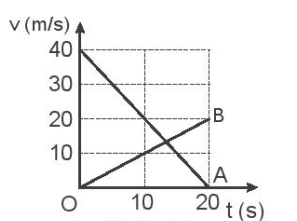
\includegraphics[width=0.6\linewidth]{../figs/VN10-2023-PH-TP0003-10}
	\end{center}
\end{minipage}

}
\hideall{
\begin{enumerate}[label=\alph*)]
	\item Gia tốc của mỗi vật:
	\begin{align*}
		\begin{cases}
			a_A=\frac{0-40}{20}=\SI{-2}{\meter/\second^2}\\
			a_B=\frac{20-0}{20}=\SI{1}{\meter/\second^2}
		\end{cases}
	\end{align*}
Phương trình vận tốc của mỗi vật:
\begin{align*}
	\begin{cases}
		v_A=40-2t\quad\left(\si{\meter/\second}\right)\\
		v_B=t\quad\left(\si{\meter/\second}\right)
	\end{cases}
\end{align*}
Hai vật có cùng vận tốc $v_A=v_B\Rightarrow t\approx\SI{13.3}{\second}$.
	\item Phương trình chuyển động của hai vật:
	$d_1=40t-t^2$; $d_2=78+0,5t^2$.
	\item Hai vật gặp nhau ở vị trí cách A một đoạn $\SI{81.5}{\meter}$.
\end{enumerate}
}


\item \mkstar{3}\\
{Thả một hòn đá rơi từ miệng một cái hang sâu xuống đến đáy. Sau $\SI{4}{\second}$ kể từ lúc bắt đầu thả thì nghe tiếng hòn đá chạm vào đáy. Tính chiều sâu của hang. Biết tốc độ truyền âm trong không khí là $\SI{330}{\meter/\second}$. Lấy $g=\SI{9.8}{\meter/\second^2}$.

}
\hideall{
	Thời gian hòn đá rơi:
	$$t=\sqrt{\dfrac{2h}{g}}+\dfrac{h}{v_a}\Rightarrow h=\SI{70.3}{\meter}.$$
}

\item \mkstar{3}\\
{Một cầu thủ bóng rổ cao $\SI{2}{\meter}$ đứng cách xa rổ $\SI{10}{\meter}$ theo phương nằm ngang để tập ném bóng vào rổ. Biết miệng rổ ở độ cao $\SI{3.05}{\meter}$. Hỏi người đó phải ném bóng từ độ cao ngang đầu với vận tốc theo phương $\SI{45}{\degree}$ có độ lớn bằng bao nhiêu để bóng rơi vào rổ? Lấy $g=\SI{9.8}{\meter/\second^2}$.

}
\hideall{
	\begin{center}
		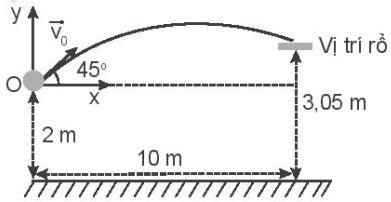
\includegraphics[width=0.4\linewidth]{../figs/VN10-2023-PH-TP0003-12}
	\end{center}
Chọn hệ trục toạ độ $Oxy$ như hình vẽ.\\
Theo phương $Ox$:
$$x=v_0t\cos\SI{45}{\degree}=\dfrac{\sqrt{2}}{2}v_0t\quad\left(\si{\meter}\right)$$
Theo phương $Oy$:
$$y=v_0t\sin\SI{45}{\degree}-\dfrac{1}{2}\cdot gt^2=\dfrac{\sqrt{2}}{2}v_0t-5t^2 \quad\left(\si{\meter}\right).$$
Để bóng rơi trúng rổ thì $x=\SI{10}{\meter}; y=\SI{1.05}{\meter} \Rightarrow v_0\approx\SI{10.57}{\meter/\second}$.
}
\end{enumerate}